\documentclass[17pt,xcolor=dvipsnames,table,dvipdfmx]{beamer}

\usepackage{slide}
\usepackage{appendixnumberbeamer}

\usepackage{math_macros}

\usepackage{import}
\usepackage{url}
\usepackage{diagbox}
\usepackage{array,colortbl}
\usepackage{hyperref}
% \hypersetup{
%     colorlinks=true,
%     citebordercolor=blue,
%     linkbordercolor=blue,
%     urlbordercolor=blue,
%     %citecolor=black,
% }

\usepackage{booktabs}

\newcommand{\comment}[2]{\textcolor{green!35!black}{#1 \fbox{\scalebox{0.4}{#2}}}}

% 引用
\usepackage[backend=bibtex, sorting=none]{biblatex}
\addbibresource{./references.bib}
% 脚注に引用文献の情報を強引に乗せる
\newcommand*{\mycite}[1]{\parencite{#1} \citeauthor{#1} (\citeyear{#1})}
\renewcommand*{\footcite}[1]{\footnote{\mycite{#1}}}
\AtBeginBibliography{\scriptsize}

\title{MP3 (aka MPEG1-Layer3)}
\author[aikiriao]{aikiriao}
\date{2024.3.XX}

\begin{document}
\maketitle

\begin{frame}[c]
    \frametitle{あらすじ}
    % \tableofcontents[hideallsubsections]
    \tableofcontents
\end{frame}

\section{成立経緯}
\section{構造}

\begin{frame}[c]
    \frametitle{MP3のエンコーダ構造}
    \begin{figure}
        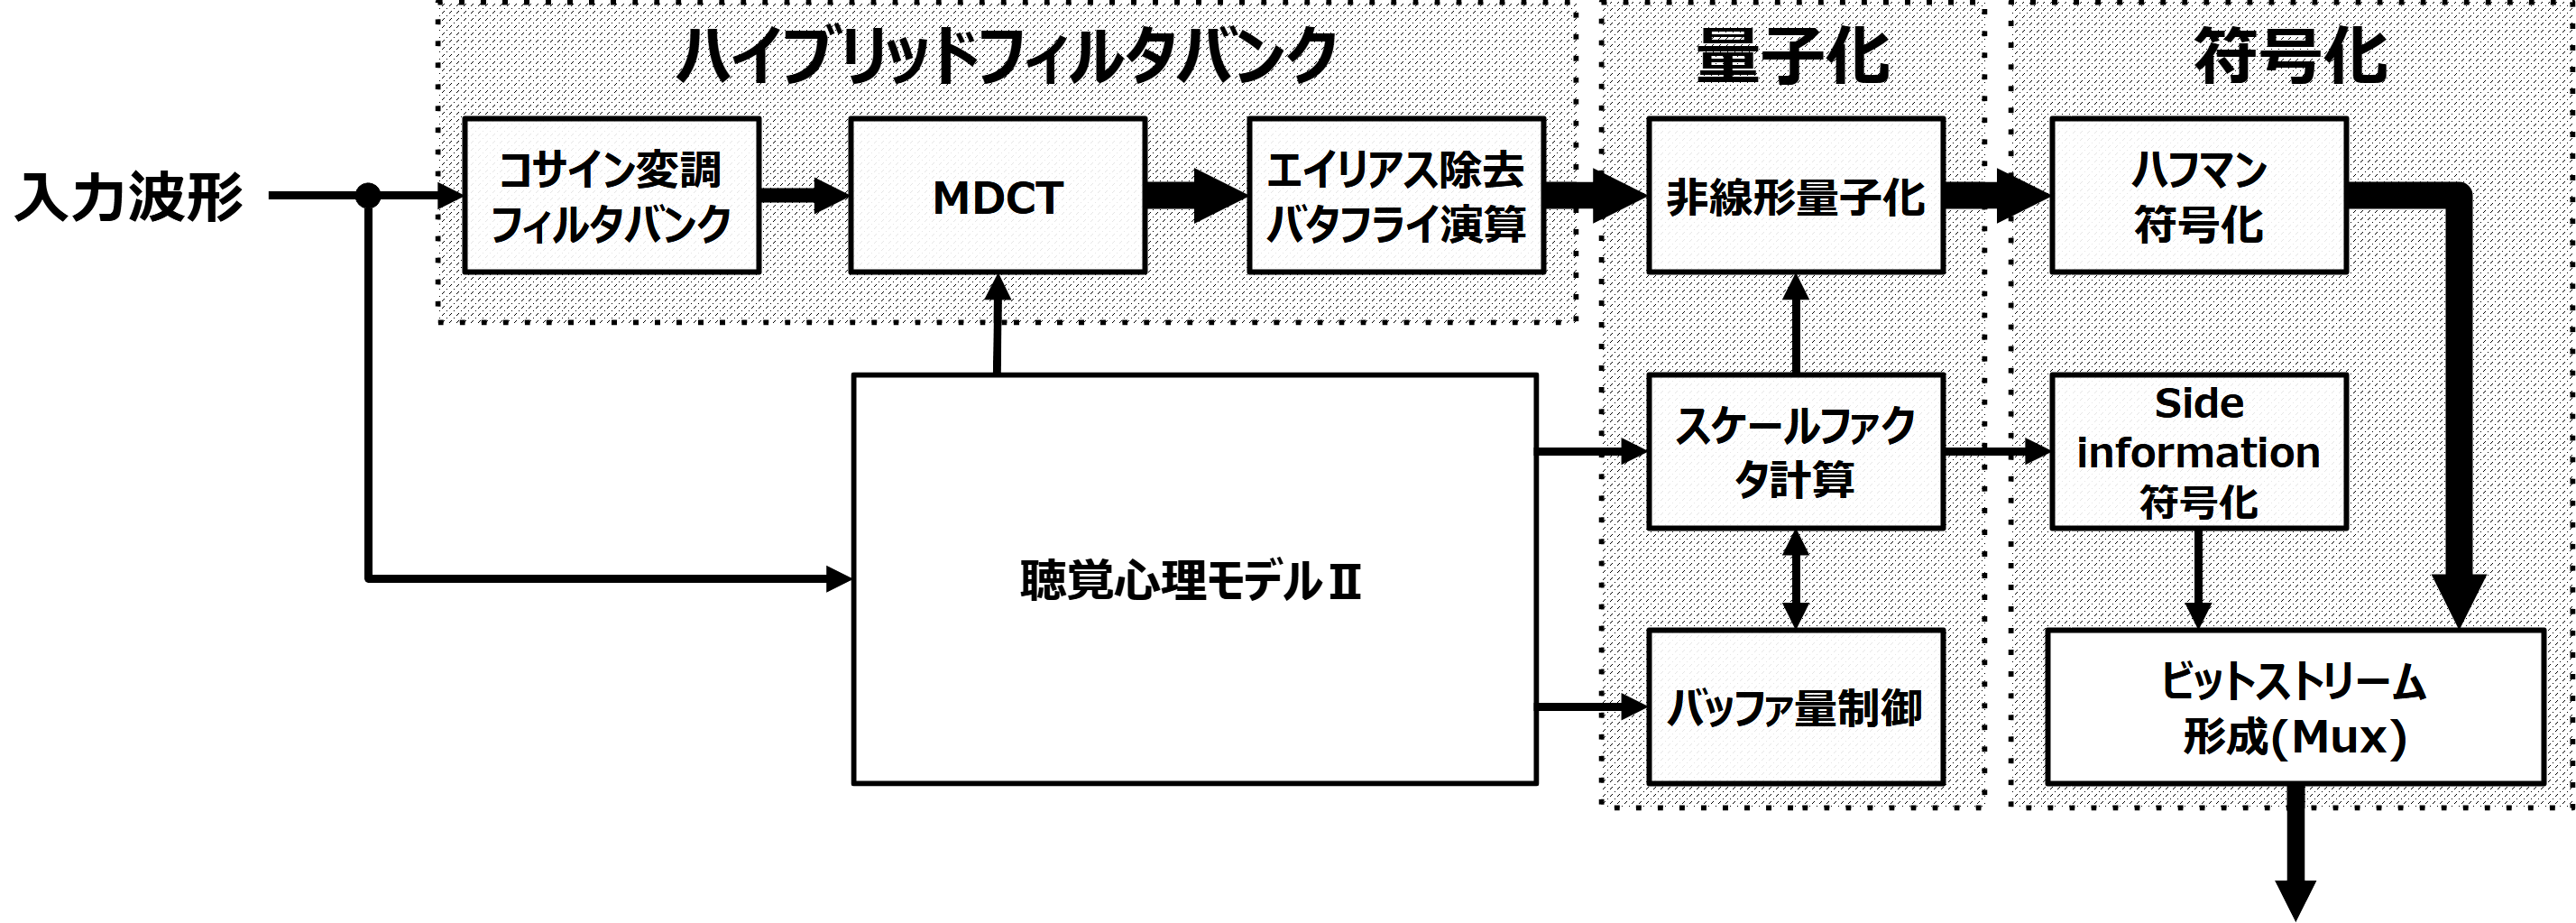
\includegraphics[width=115mm]{./figs/mp3_encoder_struct.png}
    \end{figure}
\end{frame}

\begin{frame}[c]
    \frametitle{MP3のデコーダ構造}
    \begin{figure}
        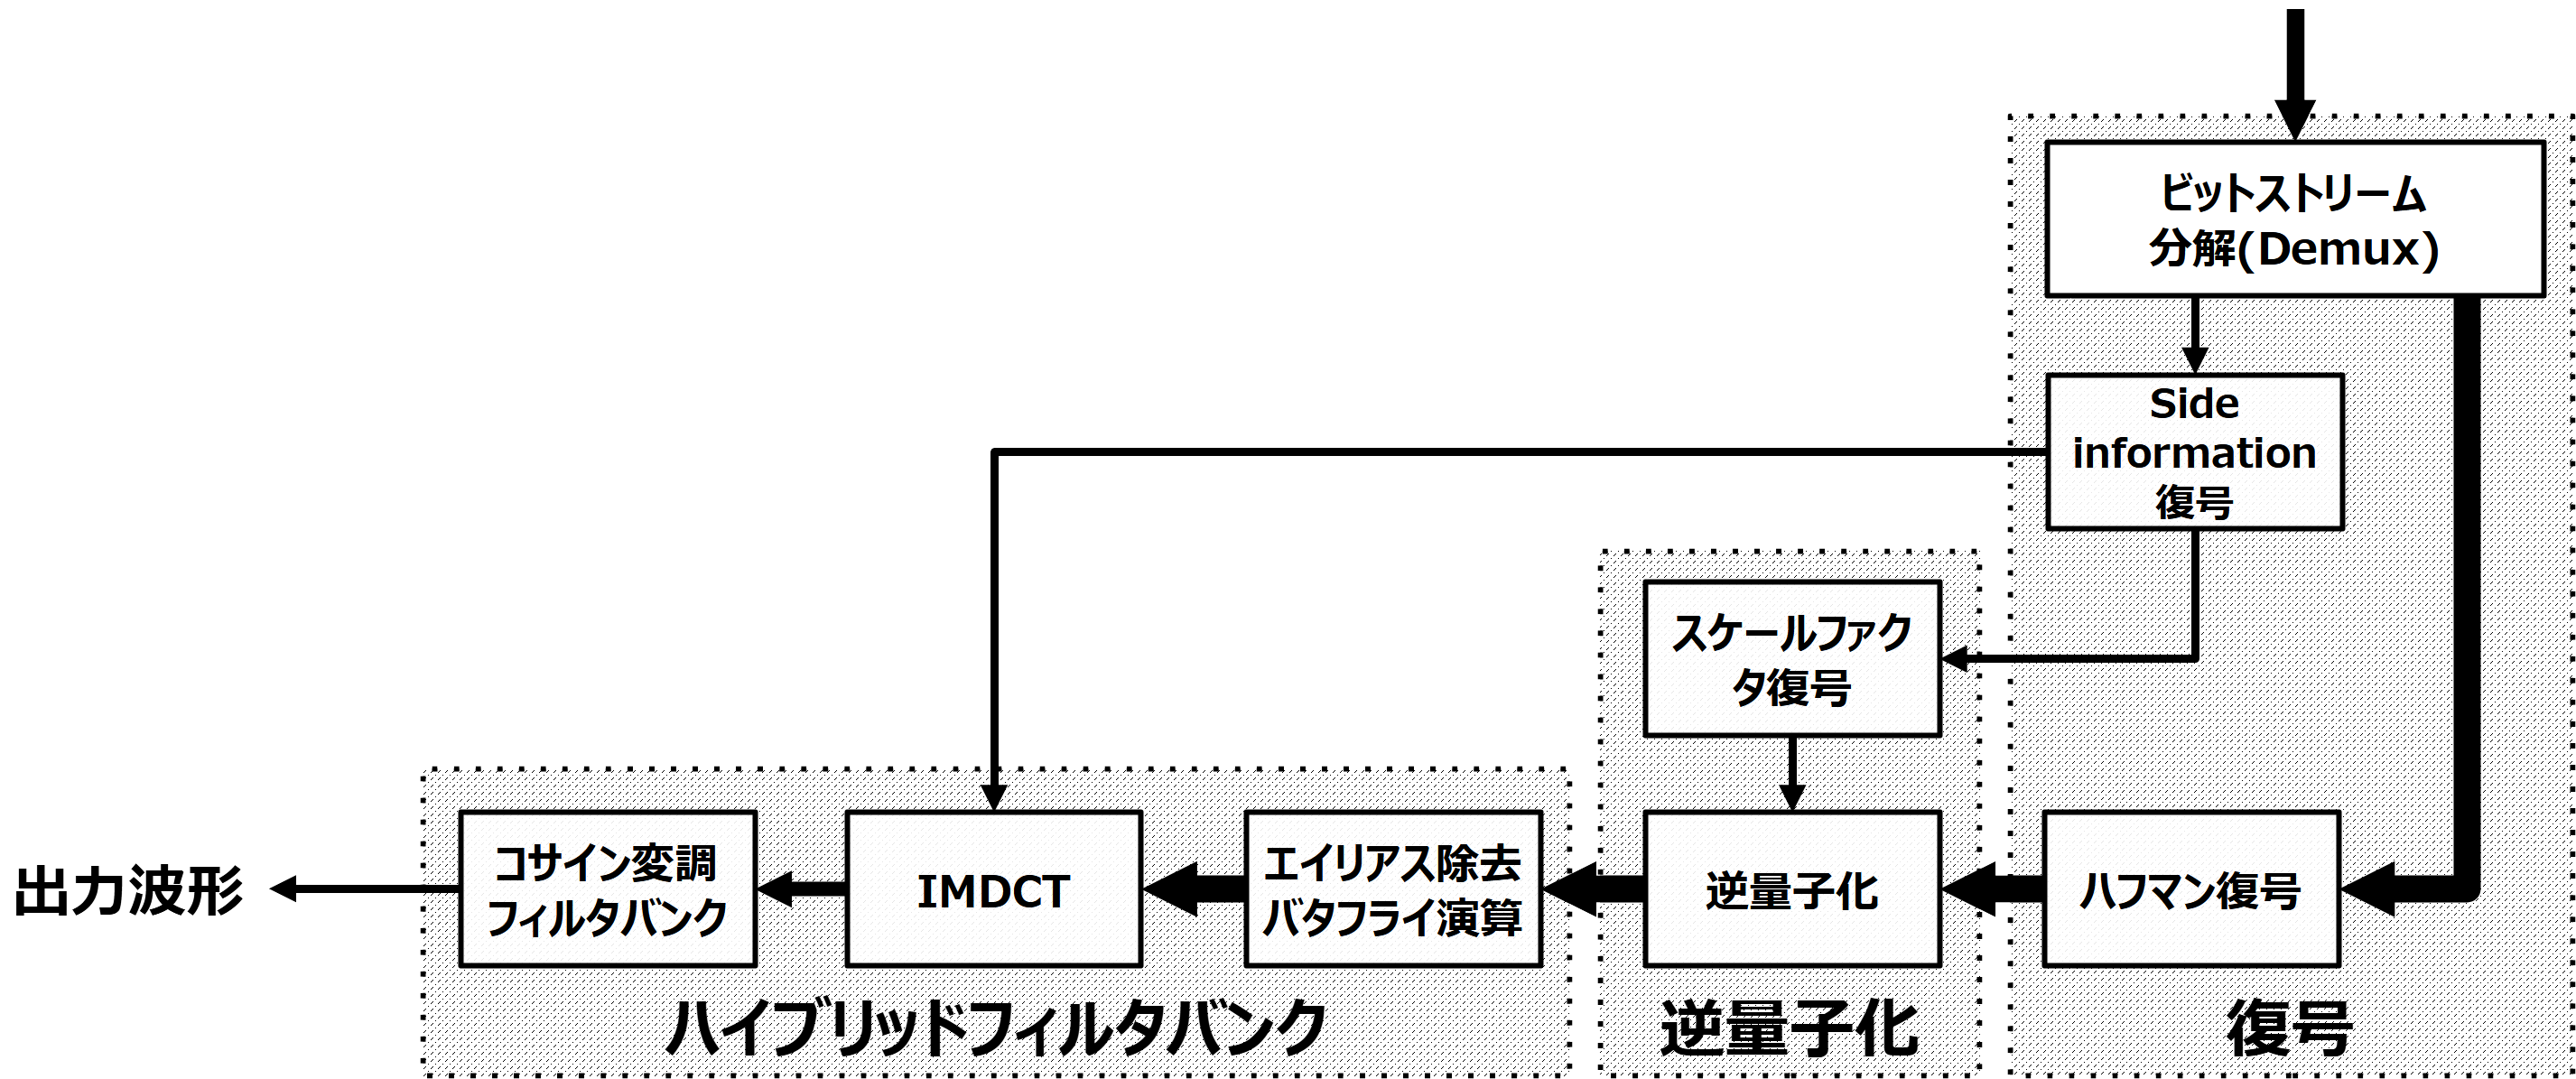
\includegraphics[width=115mm]{./figs/mp3_decoder_struct.png}
    \end{figure}
\end{frame}

\section{要素技術}
\subsection{ハイブリッドフィルタバンク}
\subsubsection{コサイン変調フィルタバンク}
\subsubsection{MDCT}
\subsubsection{エイリアス削除バタフライ演算}
\subsection{量子化}
\subsubsection{非線形量子化}
\subsubsection{スケールファクタ計算}
\subsection{符号化}
\subsection{ハフマン符号}
\subsection{聴覚モデル}

\end{document}
